% This is samplepaper.tex, a sample chapter demonstrating the
% LLNCS macro package for Springer Computer Science proceedings;
% Version 2.20 of 2017/10/04
%
\documentclass[runningheads]{llncs}
%
\usepackage{graphicx}
% Used for displaying a sample figure. If possible, figure files should
% be included in EPS format.
%
% If you use the hyperref package, please uncomment the following line
% to display URLs in blue roman font according to Springer's eBook style:
% \renewcommand\UrlFont{\color{blue}\rmfamily}

\begin{document}
%
\title{Powered by Blockchain: Next-Generation Energy Markets}
%
%\titlerunning{Abbreviated paper title}
% If the paper title is too long for the running head, you can set
% an abbreviated paper title here
%
\author{Martin Ledl}
%
\authorrunning{M. Ledl}
% First names are abbreviated in the running head.
% If there are more than two authors, 'et al.' is used.
%
\institute{Technical University of Vienna, Austria}
%
\maketitle              % typeset the header of the contribution
%
\begin{abstract}
The abstract should briefly summarize the contents of the paper in
150--250 words.

\keywords{Blockchain  \and Decentralized Energy Markets \and Decentralized Energy Trading \and Smart Grid}
\end{abstract}
%
%
%
\section{Introduction}

\section{Principles}

\subsection{Blockchain}

\subsection{Smart Grid}

\section{Energy Markets Today}
In order to be able to understand what problems currently exist and which could be tackled by application of Blockchain technology, it is very important to understand how electricity is traded nowadays and which parties are involved. Moreover, this is important to get a look into the challenges with the current system and which challenges will arise by the application of Blockchain technology or the implementation of a smart grid in general.

\subsection{Current Network Topology and Players}
The electricity system is made up of the physical infrastructure used for generation, distribution and transportation as well as the energy market itself. Therefore, people usually buy electricity not directly from generators itself, but by a wholesale company in between. Besides purchasing electricity there are further fees for using the physical infrastructure itself which cover among others maintenance costs of the grid.
This physical grid can be roughly divided into electricity generators and means of electricity transportation. Such a transportation system further consists of systems which are responsible for long-distance energy transmission and distribution systems which aim for connecting industrial and private customers to the grid in order to be able to supply them with electricity. Furthermore, there are different national or sub-national transmission system operators and distribution system operators that are responsible for maintaining the physical infrastructure and ensure stable energy distribution (e.g. for Vienna there are the “Wiener Netze”). Moreover, there are interconnections between grids also across national borders to have alternative in ensuring the electricity demand and supply. \cite{eu_energy_market}
For the other components of a electricity system, the energy market, there are various entities interacting with each other.

\subsubsection{Electricity Suppliers} buy electricity directly from energy generators and finally resell it to customers. Thus, industrial customer and residential customers usually do not purchase electricity directly from generators.

\subsubsection{Consumers} can be industrial or residential consumers and buy electricity from suppliers.

\subsection{Electricity generators} are responsible for actually generating electricity from various sources. The European Union differentiates between two types of electricity generators, firm-capacity and variable-capacity generators. Firm-capacity generators reliably deliver electricity and can be adjusted or turned on/off according to the current demand (e.g. coal, nuclear, gas, hydro with dam, biomass, etc.). Variable-capacity generators on the other hand depend on the current environmental state as they leverage wind or sunlight for example and therefore only generate electricity at certain times.  Moreover, the flexibility of firm-capacity generators varies a lot where hydro power is the most and nuclear power the least flexible with respect to latency from power on until actual energy is generated.
To underline the importance to develop a grid that can serve electricity in a stable manner with less firm-capacity generators, having a look at members of the two generator classes reveals that the firm-capacity generators contain fossil fuel (e.g. coal, natural gas, etc.) which reserve will be exhausted in a couple of decades. This will decrease the amount of energy source that can serve higher energy demand within relatively shot amount of time and therefore, the importance of more reliable integration of variable-capacity generators (e.g. all sort of renewable energy) strongly increases. This should also be a motivation that drives the restructuring and investment process in the current energy system. Besides that, burning of fossil fuels emits carbon dioxide into the atmosphere which is currently one of the main drivers of global warming. \cite{eu_energy_market}

\subsubsection{Regulators} define clear rules that has to be followed by all market entities in order to keep the market and its prices stable and make it work as it currently is. Moreover, regulators keep track if the electricity market works as it should. The Agency for Cooperation of Energy Regulators defines the network codes at EU level. Those network codes define guidelines for transnational electricity markets and networks. On national level, independent regulators set operational rules for electricity markets.

\subsubsection{Transmission System Operators} are in charge of the long-distance electricity transportation and of maintaining the transportation system and further investments in it in order to enlarge or restructure its topology. Thus, they ensure the systems stability and are therefore paid by other entities for using their infrastructure for electricity transportation.

\subsubsection{Distributions System Operators} earn money by distributing the electricity, which has been transported over a transmission system operator’s infrastructure, to the customer. \newline

The physical infrastructure of transmission and distribution networks is connected to electricity consumers and generators the electric grid. This network aims for keeping balance between demand and supply of electricity within the grid. Such stability guarantees that there is no lack of electricity at no point of time for example. Another really notable aspect is that the electricity flow within the grid cannot be controlled and due to physical laws, the electricity flows along the path of lowest resistance. Thus, *MENTION ELECTRICITY MIXTURE FROM BELOW.
The consumed electricity is generated by different systems that vary greatly in their size and scale. A generator can be a nuclear, coal or large hydro power plant, but also rather small-scale photovoltaic systems. 


\subsection{Current Energy Markets}
In the European Union, market types depend on their geographical location and vary in their size and level from transnational wholesale markets to local retail markets. In a traditional retail market, suppliers offer contracts which cover national regulators’ rules and consumers usually choose a suitable contract offered by a supplier of their choice. Suppliers resell energy from generating entities and are responsible for invoicing the offered electricity. Such contracts state the electricity’s origin as well as fees which support certain policies and network investments.
Wholesale markets bring together electricity generators, suppliers and large industrial consumers under a different pricing schema as for residential customers. Furthermore, wholesale energy markets are coupled on a transnational regional level to increase flexibility and be able to address demand across national borders.\cite{eu_energy_market}

\subsection{Balancing Supply and Demand}
The key equation for balance is that the electrical supply must be equal to the demand in order to have a stable network without shortages. The base amount of electricity is served by variable-capacity generators and demand peaks are addressed using firm-capacity generators due to their flexibility. An increase in variable capacity (increase in renewable systems) has also led to an increase in firm capacity to ensure stability. Demand and supply balancing in the European Union are done using a three-level reserve system, where the different levels have increased supply latency. Furthermore, variable capacity is prioritized and often meets the required demand which results in lower market share for firm capacity and therefore such generators earn less money these days. Nevertheless, the are most important in times of supply shortages. \cite{eu_energy_market}

\subsection{Arising Challenges}
The European Union \cite{eu_energy_market} stated in 2016 that there are a couple of challenges that need to be addressed by the future electricity system. First of all, the general electricity demand is increasing within the European Union due to the ongoing electrification (e.g. spread of electrical cars). Moreover, there is a huge aim for reduction of $CO_2$ emissions by generating electricity from variable renewable sources. This results in an increase of electricity transportation due to the increase of variable generators.\newline
Furthermore, the number of private prosumers is increasing and therefore more potential consumer generate a certain amount of energy themselves which results in a decrease in grid consumption and less revenue for conventional generators and grid operators. Unfortunately, this can lead to an increase in electricity prices and grid fees for regular consumers. \newline
Those challenges need to be effectively and efficiently tackled in the close future and therefore energy service companies are currently developing enhanced electrical systems that can address the current drive of energy generation and consumption in a more suitable way. Such adoptions require massive investments of local, national and transnational level in order to provide network resilience and competitive pricing for all network entities.\cite{eu_energy_market}

\textbf{TODO: write a few sentences in order to come to smart grid, microgrids and blockchains}


\section{Blockchain in the Energy Sector}

\section{Conclusion}

\subsection{A Subsection Sample}
Please note that the first paragraph of a section or subsection is
not indented. The first paragraph that follows a table, figure,
equation etc. does not need an indent, either.

Subsequent paragraphs, however, are indented.

\subsubsection{Sample Heading (Third Level)} Only two levels of
headings should be numbered. Lower level headings remain unnumbered;
they are formatted as run-in headings.

\paragraph{Sample Heading (Fourth Level)}
The contribution should contain no more than four levels of
headings. Table~\ref{tab1} gives a summary of all heading levels.

\begin{table}
\caption{Table captions should be placed above the
tables.}\label{tab1}
\begin{tabular}{|l|l|l|}
\hline
Heading level &  Example & Font size and style\\
\hline
Title (centered) &  {\Large\bfseries Lecture Notes} & 14 point, bold\\
1st-level heading &  {\large\bfseries 1 Introduction} & 12 point, bold\\
2nd-level heading & {\bfseries 2.1 Printing Area} & 10 point, bold\\
3rd-level heading & {\bfseries Run-in Heading in Bold.} Text follows & 10 point, bold\\
4th-level heading & {\itshape Lowest Level Heading.} Text follows & 10 point, italic\\
\hline
\end{tabular}
\end{table}


\noindent Displayed equations are centered and set on a separate
line.
\begin{equation}
x + y = z
\end{equation}
Please try to avoid rasterized images for line-art diagrams and
schemas. Whenever possible, use vector graphics instead (see
Fig.~\ref{fig1}).

\begin{figure}
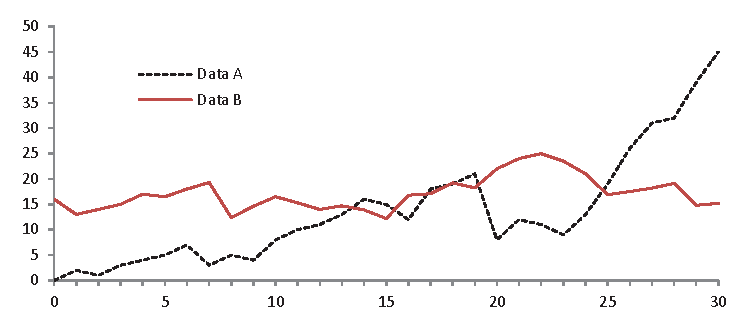
\includegraphics[width=\textwidth]{fig1.eps}
\caption{A figure caption is always placed below the illustration.
Please note that short captions are centered, while long ones are
justified by the macro package automatically.} \label{fig1}
\end{figure}

\begin{theorem}
This is a sample theorem. The run-in heading is set in bold, while
the following text appears in italics. Definitions, lemmas,
propositions, and corollaries are styled the same way.
\end{theorem}
%
% the environments 'definition', 'lemma', 'proposition', 'corollary',
% 'remark', and 'example' are defined in the LLNCS documentclass as well.
%
\begin{proof}
Proofs, examples, and remarks have the initial word in italics,
while the following text appears in normal font.
\end{proof}
For citations of references, we prefer the use of square brackets
and consecutive numbers. Citations using labels or the author/year
convention are also acceptable. The following bibliography provides
a sample reference list with entries for journal
articles~\cite{ref_article1}, an LNCS chapter~\cite{ref_lncs1}, a
book~\cite{ref_book1}, proceedings without editors~\cite{ref_proc1},
and a homepage~\cite{ref_url1}. Multiple citations are grouped
\cite{ref_article1,ref_lncs1,ref_book1},
\cite{ref_article1,ref_book1,ref_proc1,ref_url1}.
%
% ---- Bibliography ----
%
% BibTeX users should specify bibliography style 'splncs04'.
% References will then be sorted and formatted in the correct style.
%
% \bibliographystyle{splncs04}
% \bibliography{mybibliography}
%
\begin{thebibliography}{8}
\bibitem{eu_energy_market}
European Parliament Homepage, \url{https://www.europarl.europa.eu/RegData/etudes/BRIE/2016/593519/EPRS\_BRI(2016)593519\_EN.pdf}. Last accessed 7 Nov 2020

\bibitem{ref_article1}
Author, F.: Article title. Journal \textbf{2}(5), 99--110 (2016)

\bibitem{ref_lncs1}
Author, F., Author, S.: Title of a proceedings paper. In: Editor,
F., Editor, S. (eds.) CONFERENCE 2016, LNCS, vol. 9999, pp. 1--13.
Springer, Heidelberg (2016). \doi{10.10007/1234567890}

\bibitem{ref_book1}
Author, F., Author, S., Author, T.: Book title. 2nd edn. Publisher,
Location (1999)

\bibitem{ref_proc1}
Author, A.-B.: Contribution title. In: 9th International Proceedings
on Proceedings, pp. 1--2. Publisher, Location (2010)

\bibitem{ref_url1}
LNCS Homepage, \url{http://www.springer.com/lncs}. Last accessed 4
Oct 2017
\end{thebibliography}
\end{document}
